\documentclass[conference]{IEEEtran}
\IEEEoverridecommandlockouts
\usepackage{cite}
\usepackage{amsmath,amssymb,amsfonts}
\usepackage{algorithmic}
\usepackage{graphicx}
\usepackage{textcomp}
\usepackage{xcolor}
\usepackage{booktabs}

\newcommand{\rupee}{\text{Rs.}}
\graphicspath{{figures/}}

\def\BibTeX{{\rm B\kern-.05em{\sc i\kern-.025em b}\kern-.08em
    T\kern-.1667em\lower.7ex\hbox{E}\kern-.125emX}}

\begin{document}

\title{A Comparative Analysis Framework for P2P Energy Trading in Community Microgrids}

\author{
\IEEEauthorblockN{Alen Shaju, Aarav Kumar, Anshu Singh, Urishita Gupta, and VSKV Harish}
\IEEEauthorblockA{\textit{Department of Electrical Engineering} \\
\textit{Netaji Subhas University of Technology (NSUT)}\\
New Delhi, India \\
vskvharish@ieee.org}
}

\maketitle

\begin{abstract}
This paper presents a modular comparative analysis framework for evaluating peer-to-peer (P2P) energy trading mechanisms in community microgrids. Four settlement strategies (conventional billing, Bill Sharing, Mid-Market Ratio, and Supply-Demand Ratio with Demand-Side Management) are benchmarked on identical community profiles.
Standardized metrics such as cost savings and a fairness index quantifying consumer-prosumer equity are used. An iterative distributed algorithm resolves the closed-loop price-demand feedback shown in incorporation of DSM. The framework is run across community sizes from $N=7$ to $N=30$ households, demonstrating that MMR and static SDR tends to penalize prosumers while when demand-side management is incorporated with SDR pricing, the highest community savings and fairness is achieved simultaneously, leading to positive outcomes for both consumers and prosumers across all configurations tested.
\end{abstract}

\begin{IEEEkeywords}
Peer-to-peer energy trading, microgrid pricing, supply-demand ratio, demand-side management, community energy markets
\end{IEEEkeywords}

%====================================================================
\section{Introduction}

Global renewable generation capacity reached 4,448~GW in 2024, with photovoltaic (PV) installations accounting for 75\% of new additions~\cite{irena2025}. As rooftop PV proliferate, community microgrids have emerged as a localized solution for coordinating distributed energy resources (DERs) through decentralized Peer-to-Peer (P2P) energy sharing and trading~\cite{sousa2019}. P2P trading refers to an internal electricity market where prosumers and consumers exchange energy at prices determined by aggregated community supply and demand, with continuous grid interconnection ensuring reliability~\cite{zhou2023}. The fundamental concept is illustrated in Fig.~\ref{fig:concept}.

\begin{figure}[t]
    \centering
    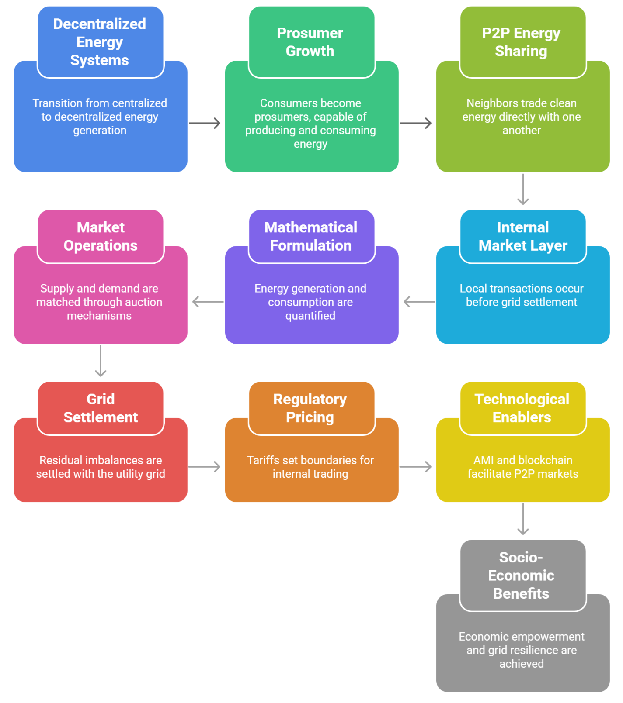
\includegraphics[width=\columnwidth]{fig1.png}
    \caption{Concept of P2P energy sharing and trading.}
    \label{fig:concept}
\end{figure}

\subsection{Limitations of Existing Approaches}

P2P systems can be classified along two dimensions: sharing architecture (centralized, decentralized, distributed) and market design (cost-sharing, auction-based, ratio-based deterministic pricing)~\cite{domenech2022}.

\textit{Cost-sharing mechanisms} such as the Bill Sharing Mechanism (BSM) pool community resources and redistribute costs based on allocation rules~\cite{long2017}. 
Mechanisms such as BSM are simpler to implement but if real-time load shifting is incorporated BSM fails to incentivize it and lack temporal granularity ~\cite{zhang2018}.


\textit{Auction-based mechanisms} require significant communication overhead and is more complex to implement in practice as it requires the various peers to submit their bids, which leads to a market-clearing price being determined~\cite{huang2025, zhang2024}. Game-theoretic formulations~\cite{long2019, tushar2019} share similar complexity concerns for practical deployment.

\textit{Ratio-based deterministic pricing}, they include strategies like Mid-Market Ratio (MMR) and Supply-Demand Ratio, they derive internal prices directly from aggregate power quantities and do not involve strategic bidding ~\cite{bogensperger2021, teotia2020}. This however, leads to the high yielding prosumers to be penalized and consumers  benefiting. ~\cite{alfaverh2023} Quantitative analysis by Dwivedi et al.~\cite{dwivedi2022} demonstrated that conventional P2P mechanisms can reduce prosumer revenues by 8-15\% compared to direct grid export, discouraging sustained market participation. 

Table~\ref{tab:literature} summarizes significant recent works. 
The literature typically addresses the various pricing mechanisms (such as SDR, MMR, BS), DSM ~\cite{liu2017} or uncertanity and fairness concerns in isolation. A unified comparative analysis framework with configurable parameters which allows to provide actionable recommendations based on community composition remains underdeveloped.

\begin{table*}[t]
\caption{Summary of Significant Works on P2P Energy Trading Architectures}
\label{tab:literature}
\centering
\footnotesize
\begin{tabular}{p{2.2cm}p{2cm}p{2.5cm}p{1.5cm}p{2cm}p{1.8cm}p{2.5cm}}
\toprule
\textbf{Source} & \textbf{Market Model} & \textbf{Pricing Mechanism} & \textbf{DSM} & \textbf{Optimization} & \textbf{Uncertainty} & \textbf{Test System} \\
\midrule
Liu (2017) & Centralized P2P & SDR-based pricing & Yes & Iterative optim. & Deterministic & China Southern Grid \\
Jia (2023) & Receding-horizon & Interval matching + CVaR & Yes & Nash bargaining & Prediction intervals & IEEE 13 \& 123 bus \\
Kanakadhurga (2024) & Residential $\mu$grid & SDR + RTP + Double Auction & Yes & Binary Dragonfly & EV uncertainty & 4-home microgrid \\
Ali (2022) & Decentralized P2P & Double auction & Limited & Game-theoretic & Forecast-based & Community microgrid \\
Veeraswamy (2024) & Distributed P2P & Mid-Market Rate & No & Auction clearing & None & Residential community \\
\bottomrule
\end{tabular}
\end{table*}

\subsection{Contributions}

While the literature has explored the various pricing mechanisms and even the effects of incorporating DSM, the present work makes the following distinct contributions:
\begin{enumerate}
    \item A \textit{modular comparative analysis framework} that evaluates multiple P2P settlement mechanisms (Conventional, BSM, MMR, SDR, SDR-DSM) on identical community profiles using standardized metrics (cost savings and a fairness index quantifying consumer-vs-prosumer equity), enabling systematic benchmarking under controlled conditions.
    \item Study of price-responsive DSM with SDR pricing through a distributed iterative algorithm, resolving the closed-loop price--demand feedback that static SDR formulations do not address.
    \item An \textit{equity-focused evaluation} across community sizes ($N=7$ to $N=30$) demonstrating that MMR and static SDR consistently penalize prosumers, while the integration of demand-side management significantly improves both community savings and fairness simultaneously.
\end{enumerate}

%====================================================================
\section{System Model}

\subsection{Community Microgrid Architecture}

The framework is parameterized for an arbitrary number of households $N$ with configurable prosumer-consumer composition and PV sizing categories. Consider a community microgrid with $N$ households comprising PV prosumers $\mathcal{P}$ and consumers $\mathcal{C}$, where $\mathcal{N} = \mathcal{P} \cup \mathcal{C}$. An Energy Service Provider (ESP) acts as the central coordinator for market clearing and settlement. For this case study we use $N = 10$ as a representative case. The framework is modular and it generalizes to larger communities without structural modification. The simulation horizon spans $H$ discrete time slots of duration $\Delta t$ hours.

For household $n \in \mathcal{N}$ at time slot $t$, the net power is:
\begin{equation}
    P_{n,t}^{\text{net}} = D_{n,t} - G_{n,t}
    \label{eq:net_power}
\end{equation}
where $D_{n,t}$ is the electricity demand and $G_{n,t}$ is PV generation (with $G_{n,t} \equiv 0$ for consumers $n \in \mathcal{C}$). Self-consumption, import, and export powers are:
\begin{equation}
    P_{n,t}^{\text{self}} = \min(D_{n,t},\; G_{n,t})
    \label{eq:self_consumption}
\end{equation}
\begin{equation}
    P_{n,t}^{\text{im}} = \max(P_{n,t}^{\text{net}},\; 0), \quad P_{n,t}^{\text{ex}} = \max(-P_{n,t}^{\text{net}},\; 0)
    \label{eq:import_export}
\end{equation}

The grid buying tariff $\pi^{\text{buy}}$ and selling tariff $\pi^{\text{sell}}$ set the upper and lower bounds for internal P2P prices. Community-level reference tariffs are:
\begin{equation}
    \bar{\pi}^{\text{buy}} = \frac{1}{N}\sum_{n=1}^{N}\pi_n^{\text{buy}}, \quad \bar{\pi}^{\text{sell}} = \frac{1}{|\mathcal{P}|}\sum_{n \in \mathcal{P}}\pi_n^{\text{sell}}
    \label{eq:ref_tariffs}
\end{equation}

%====================================================================
\section{P2P Pricing Mechanisms}

\subsection{Bill Sharing Mechanism (BSM)}

The BSM pools community resources over the billing period and computes constant ex-post prices. Total community import and export energies are:
\begin{equation}
    E^{\text{buy}} = \sum_{t} P_t^{\text{buy}} \cdot \Delta t, \quad E^{\text{sell}} = \sum_{t} P_t^{\text{sell}} \cdot \Delta t
    \label{eq:bsm_energy}
\end{equation}
where $P_t^{\text{buy}} = \sum_{n} P_{n,t}^{\text{im}}$ and $P_t^{\text{sell}} = \sum_{n} P_{n,t}^{\text{ex}}$. The community's net grid interaction determines internal prices:
\begin{equation}
    \pi_t^{\text{int,buy}} = \frac{\bar{\pi}^{\text{buy}} \cdot E_{\text{grid}}^{\text{im}}}{E^{\text{buy}}}, \quad \pi_t^{\text{int,sell}} = \frac{\bar{\pi}^{\text{sell}} \cdot E_{\text{grid}}^{\text{ex}}}{E^{\text{sell}}}
    \label{eq:bsm_prices}
\end{equation}

BSM produces temporally invariant prices, which while ensuring simplicity, provides no incentive for real-time load adjustment.

\subsection{Mid-Market Ratio (MMR) Pricing}

The MMR establishes a time-varying midpoint price anchored between grid tariffs:
\begin{equation}
    \pi^{\text{mid}} = \frac{\bar{\pi}^{\text{buy}} + \bar{\pi}^{\text{sell}}}{2}
    \label{eq:mmr_mid}
\end{equation}

At each time slot, the community net balance index is:
\begin{equation}
    \eta_t = \frac{P_t^{\text{buy}} - P_t^{\text{sell}}}{P_t^{\text{buy}} + P_t^{\text{sell}}}
    \label{eq:mmr_balance}
\end{equation}

The P2P clearing price adjusts dynamically:
\begin{equation}
    \pi_t^{\text{p2p}} = \pi^{\text{mid}} + \frac{\bar{\pi}^{\text{buy}} - \bar{\pi}^{\text{sell}}}{2} \cdot \eta_t
    \label{eq:mmr_price}
\end{equation}

When community supply exceeds demand, the effective selling price is reduced proportionally as surplus energy is exported to the grid at the feed-in tariff. Conversely, during deficit periods, the buying price increases toward the retail tariff. While MMR introduces temporal price variation, it can significantly depress prosumer revenues during surplus periods.

\subsection{Supply-Demand Ratio (SDR) Based Pricing}
The Supply-Demand Ratio (SDR) captures the balance between the supply and demand at any given instant:

\begin{equation}
    \text{SDR}_t = \frac{P_t^{\text{sell}}}{P_t^{\text{buy}} + \varepsilon}
    \label{eq:sdr}
\end{equation}
 $\varepsilon$ is taken as a small constant needed for numerical stability. The SDR directly signify market dynamics as i: $\text{SDR}_t < 1$ indicates energy shortage, $\text{SDR}_t = 1$ represents balance, and $\text{SDR}_t > 1$ signals surplus.

The internal P2P prices are bound between the grid tarifs and are functions of the SDR. The selling price is:
\begin{equation}
    \pi_t^{\text{int,sell}} = \frac{\bar{\pi}^{\text{buy}} \cdot \bar{\pi}^{\text{sell}}}{(\bar{\pi}^{\text{buy}} - \bar{\pi}^{\text{sell}}) \cdot \text{SDR}_t + \bar{\pi}^{\text{sell}}}
    \label{eq:sdr_sell}
\end{equation}

The buying price is defined piecewise:
\begin{equation}
    \pi_t^{\text{int,buy}} = \begin{cases}
        \pi_t^{\text{int,sell}} \cdot \text{SDR}_t + \bar{\pi}^{\text{buy}} \cdot (1 - \text{SDR}_t), & \text{SDR}_t < 1 \\
        \bar{\pi}^{\text{sell}}, & \text{SDR}_t \geq 1
    \end{cases}
    \label{eq:sdr_buy}
\end{equation}

Similarly, the selling price \eqref{eq:sdr_sell} is clamped: $\pi_t^{\text{int,sell}} = \bar{\pi}^{\text{sell}}$ when $\text{SDR}_t \geq 1$. This formulation makes sure that : (i)~price is a monotonous function with respect to SDR, (ii) prices are bounded between $[\bar{\pi}^{\text{sell}},\; \bar{\pi}^{\text{buy}}]$, and (iii)~zero-arbitrage conditions.

\subsection{SDR with Demand-Side Management}

Demand side Management can be incorporated by the participants to increase their savings. Consider that participants can adjust consumption $x_{n,t}$ in response to price signals. Then the net power becomes:
\begin{equation}
    P_{n,t}^{\text{net}} = x_{n,t} - G_{n,t}
    \label{eq:dsm_net}
\end{equation}
A particular users discomfort to shifting their load can be modelled using a quadratic penalty ~\cite{alfaverh2023}:
\begin{equation}
    C_{n}^{\text{inc}} = \alpha_n \sum_{t=1}^{H} (x_{n,t} - D_{n,t}^{\text{ref}})^2 \cdot \Delta t
    \label{eq:inconvenience}
\end{equation}
where $D_{n,t}^{\text{ref}}$ is the initial load profile and $\alpha_n$ is the sensitivity coefficient representing their tolerance to shifting their loads. The quadratic form is a widely adopted mechanism in demand response literature~\cite{liu2017, alfaverh2023}, as large deviations from the scheduled load is penalized disproportionately, reflecting what happens in practice as minor adjustments are often tolerable but major adjustments (such as turning the dishwasher on past midnight etc.) get increasingly more inconvenient. 

Each participant independently minimizes:
\begin{equation}
    \min_{x_{n,t}} \sum_{t=1}^{H} \left[ \pi_{n,t} \cdot P_{n,t}^{\text{net}} \cdot \Delta t + \alpha_n (x_{n,t} - D_{n,t}^{\text{ref}})^2 \cdot \Delta t \right]
    \label{eq:objective}
\end{equation}
subject to:
\begin{equation}
    \sum_{t=1}^{H} x_{n,t} \cdot \Delta t = \sum_{t=1}^{H} D_{n,t}^{\text{ref}} \cdot \Delta t
    \label{eq:energy_conservation}
\end{equation}
\begin{equation}
    D_{n}^{\text{min}} \leq x_{n,t} \leq D_{n}^{\text{max}}, \quad \forall t
    \label{eq:load_bounds}
\end{equation}

Constraint~\eqref{eq:energy_conservation}  makes sure that the total energy remains conserved , ie. making sure that only load shifting is taking place and not load curtailment during DSM. Constraint~\eqref{eq:load_bounds} imposes a physical appliance-level practical bounds reflecting the practical range of  loads that can be deffered (e.g., water heaters, EV charging, washing machines).

For arriving at a market clearing price during DSM a closed loop interaction is introduced, prices depend on SDR and SDR depends on aggregate demand and then again demand depends on prices.  This feedback loop is resolved through an iterative fixed-point algorithm coordinated by the ESP.

The ESP revenue is derived from a service fee proportional to locally traded energy:
\begin{equation}
    S^{\text{ESP}} = \beta \sum_{t=1}^{H} \min(P_t^{\text{sell}},\; P_t^{\text{buy}}) \cdot \Delta t
    \label{eq:esp_revenue}
\end{equation}
where $\beta$ covers metering, communication, settlement, and losses.

To quantify equity across participant groups, the framework computes a fairness index:
\begin{equation}
    \mathcal{F} = 1 - \frac{|\Delta_{\mathcal{C}} - \Delta_{\mathcal{P}}|}{|\Delta_{\mathcal{C}}| + |\Delta_{\mathcal{P}}| + \varepsilon}
    \label{eq:fairness}
\end{equation}
where $\Delta_{\mathcal{C}}$ and $\Delta_{\mathcal{P}}$ are the  percentage cost improvements for consumers and prosumers as a group respectively (positive = benefit, negative = loss), relative to conventional billing. $\mathcal{F} = 1$ when both groups benefit equally; $\mathcal{F} \to 0$ when one group's gain comes entirely at the other's expense.

%====================================================================
\section{Distributed Settlement Algorithm}

The SDR-DSM mechanism is solved through a distributed iterative algorithm. At each iteration, the ESP aggregates prosumer schedules, computes the community SDR, and updates P2P prices. Participants then independently re-optimize their load schedules given updated prices. The process repeats until convergence.

\vspace{4pt}
\hrule\vspace{4pt}
\noindent\textbf{Algorithm 1:} Distributed SDR-DSM Settlement\\
\vspace{2pt}\hrule\vspace{4pt}
\noindent\textbf{Input:} $D_{n,t}^{\text{ref}}$, $G_{n,t}$, $\pi^{\text{buy}}$, $\pi^{\text{sell}}$, $\alpha_n$, $\epsilon_{\text{conv}}$\\
\textbf{Output:} $x_{n,t}^{*}$, $\pi_t^{\text{int,buy}}$, $\pi_t^{\text{int,sell}}$
\begin{enumerate}
    \item Initialize $x_{n,t}^{(0)} \leftarrow D_{n,t}^{\text{ref}}$ for all $n, t$; set $k \leftarrow 0$
    \item \textbf{Repeat:}
    \begin{enumerate}
        \item[(a)] ESP aggregates $P_t^{\text{sell},(k)}$, $P_t^{\text{buy},(k)}$ from $\{x_{n,t}^{(k)}\}$
        \item[(b)] Compute $\text{SDR}_t^{(k)}$ via \eqref{eq:sdr}
        \item[(c)] Update prices $\pi_t^{(k)}$ via \eqref{eq:sdr_sell}--\eqref{eq:sdr_buy}
        \item[(d)] Each participant $n$ solves \eqref{eq:objective} s.t. \eqref{eq:energy_conservation}--\eqref{eq:load_bounds} to obtain $x_{n,t}^{(k+1)}$
        \item[(e)] $k \leftarrow k + 1$
    \end{enumerate}
    \item \textbf{Until} $\max_n \|x_n^{(k)} - x_n^{(k-1)}\| < \epsilon_{\text{conv}}$
\end{enumerate}
\vspace{2pt}\hrule
\vspace{4pt}

Each peer solves the convex quadratic program with a unique minimizer for the given prices. The penalty $\alpha$ regularizes the demand response, so the optimal load adjustment to a price changes  $\delta\pi$ scales as $\mathcal{O}(\delta\pi / \alpha)$ larger the alpha the more damping there is per-iteration, therefore demand shifts and reduces the feedback gain of the composite mapping. A damping factor of 0.3 is applied to inter-iteration updates to enhance stability. A formal contraction bound is deferred to future work. Empirically, the algorithm is run for 8 iterations with $\alpha = 0.12$~\rupee$\cdot$kW$^{-1}$; the maximum load change between final iterations falls below $10^{-2}$~kW across all scenarios tested, which indicated practical convergence.

%====================================================================
\section{Simulation Setup}

\subsection{System Configuration}

The representative community microgrid taken for this study consists of $N = 10$ households which contain 3 pure consumers and 7 PV prosumers (3 small, 2 medium, 2 large). The simulation runs for 30 days at 15-minute resolution ($\Delta t = 0.25$~h), yielding 96 time slots per day and 2,880 total time steps. Table~\ref{tab:params} summarizes the key parameters.

\begin{table}[t]
\caption{Simulation Parameters}
\label{tab:params}
\centering
\begin{tabular}{lll}
\toprule
\textbf{Parameter} & \textbf{Value} & \textbf{Unit} \\
\midrule
Simulation duration & 30 & days \\
Time resolution ($\Delta t$) & 15 & min \\
Households ($N$) & 10 & -- \\
\quad Consumers & 3 & -- \\
\quad Prosumers (S/M/L) & 3/2/2 & -- \\
Consumer daily load & 4--7 & kWh/day \\
Prosumer daily load & 5--9 & kWh/day \\
PV yield & 4.5--5.5 & kWh/kWp/day \\
Grid buy tariff ($\pi^{\text{buy}}$) & 5.8752 & \rupee/kWh \\
Grid sell tariff ($\pi^{\text{sell}}$) & 3.2462 & \rupee/kWh \\
DSM discomfort coefficient ($\alpha$) & 0.12 & \rupee$\cdot$kW$^{-1}$ \\
DSM damping factor & 0.3 & -- \\
Max iterations & 8 & -- \\
ESP service fee ($\beta$) & 2 & \% \\
\bottomrule
\end{tabular}
\end{table}

The demand profile is made such that it follows a composite Gaussian shape with with morning (08:00) and evening (20:00) peaks, $\pm$5\% daily variation, and adding occasional noise per-slot. PV generation follows a clear-sky sinusoidal curve (06:00--18:00) with $\pm$15\% variability (due to external reasons such as clouds etc.). The prosumers are also categorized by their PV sizing: small (40--60\% of load), medium (80--110\%), and large (130--180\%).

\subsection{Contingency Modeling}
For modeling contingency, two types are taken into consideration: (i)~ full-day PV outages due to inverter failure (2 events/month), and (ii)~P2P trading disruptions during communication failures (3 events, 2~hours each). Affected peers settle directly with the grid.

\subsection{Software Implementation}

The simulation used Python 3.14 using NumPy for numerical computation and Pandas for handling the data. A streamlit based reccomender dashboard was developed. The iterative SDR-DSM algorithm is implemented as a custom fixed-point solver ensuring finer control and efficiency. 

%====================================================================
\section{Results and Discussion}

\subsection{Community Aggregate Power Profiles}

Fig.~\ref{fig:aggregate} shows community aggregate power profiles. The adjusted load under SDR-DSM exhibits pronounced midday advancement relative to the reference twin-peak pattern, aligning demand with PV generation. This temporal shifting mitigates midday exports and enhances local self-consumption.

\begin{figure}[t]
    \centering
    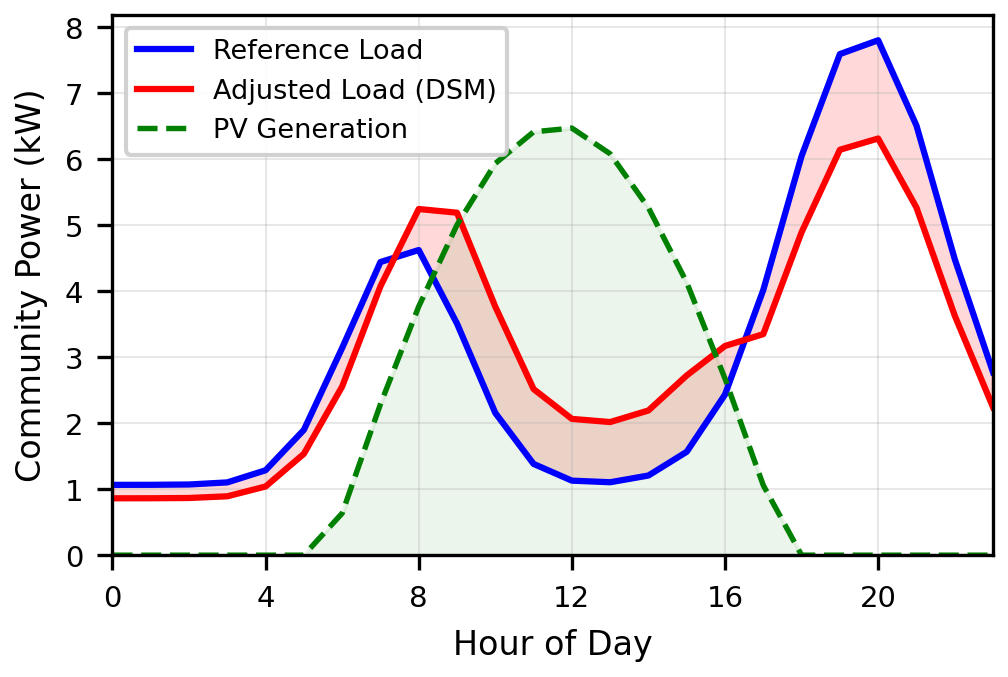
\includegraphics[width=\columnwidth]{fig7.png}
    \caption{Aggregate load profile and PV generation for the community microgrid showing reference load, adjusted load, and surplus/deficit regions.}
    \label{fig:aggregate}
\end{figure}

\subsection{Individual Load Reshaping Under SDR-DSM}

Fig.~\ref{fig:consumer_reshape} shows load reshaping for a few representative prosumers. Price signals drive participants to advance deferrable loads into midday intervals (hours 9--15) where high PV surplus produces low clearing prices, while reducing morning and evening consumption. Prosumer~1 (large PV) aggressively shifts demand toward its peak generation period, reducing its evening load substantially. Prosumer~3 (medium PV) exhibits similar but more moderate reshaping, synchronizing load with available solar output. The shaded region illustrates the magnitude of DSM-induced load shifting relative to the reference profile.

\begin{figure}[t]
    \centering
    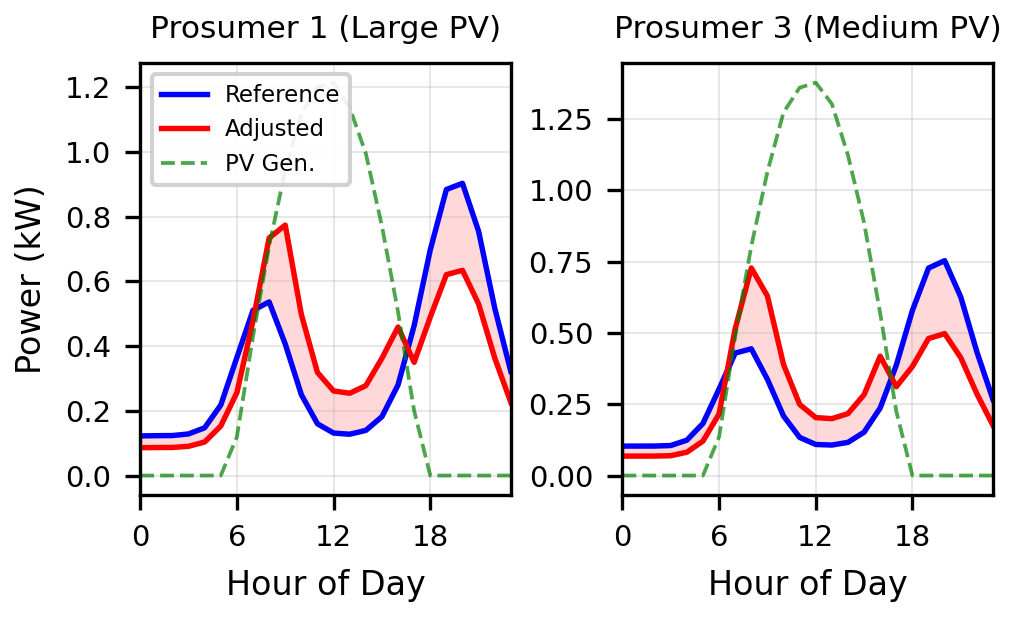
\includegraphics[width=\columnwidth]{fig8.png}
    \caption{Sample prosumer load profiles showing reference and adjusted loads under SDR-DSM pricing, with PV generation overlay.}
    \label{fig:consumer_reshape}
\end{figure}

\subsection{SDR Dynamics and Price Formation}

The SDR (Fig.~\ref{fig:sdr}) splits the operational time into 3 sections: morning deficit ($\text{SDR}_t \ll 1$), midday surplus ($\text{SDR}_t > 1$, peaking at 16.46 during 10:00--14:00), and evening deficit as PV generation stops.

\begin{figure}[t]
    \centering
    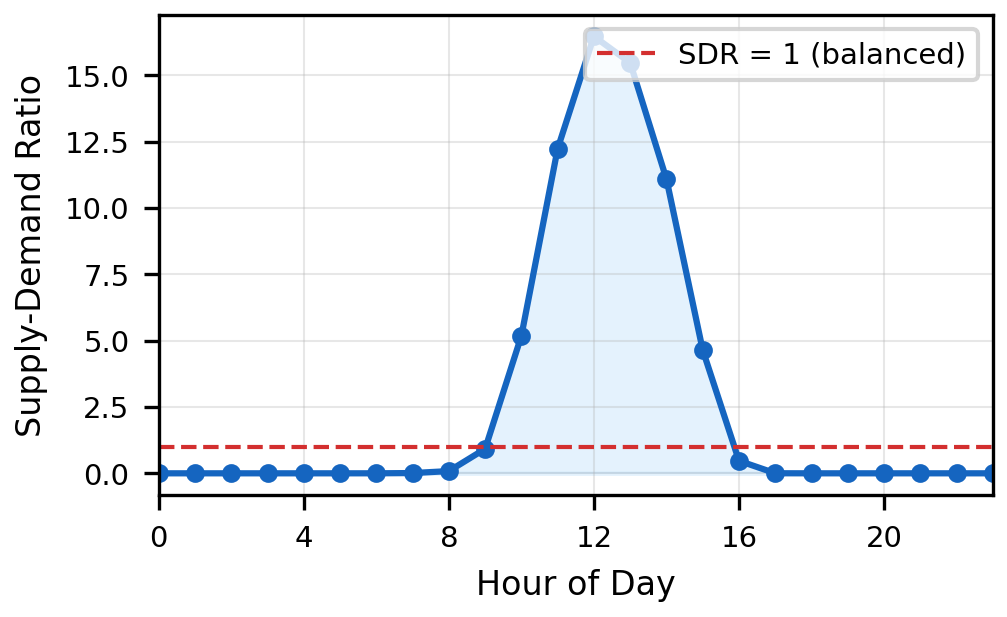
\includegraphics[width=\columnwidth]{fig11.png}
    \caption{Hourly Supply-Demand Ratio variation for the community microgrid.}
    \label{fig:sdr}
\end{figure}

Fig.~\ref{fig:prices} shows the corresponding P2P clearing prices. During peak PV periods, internal prices collapse from \rupee~5.8752/kWh to the export floor of \rupee~3.2462/kWh, serving as a natural DSM trigger while remaining strictly bounded between utility limits.

\begin{figure}[t]
    \centering
    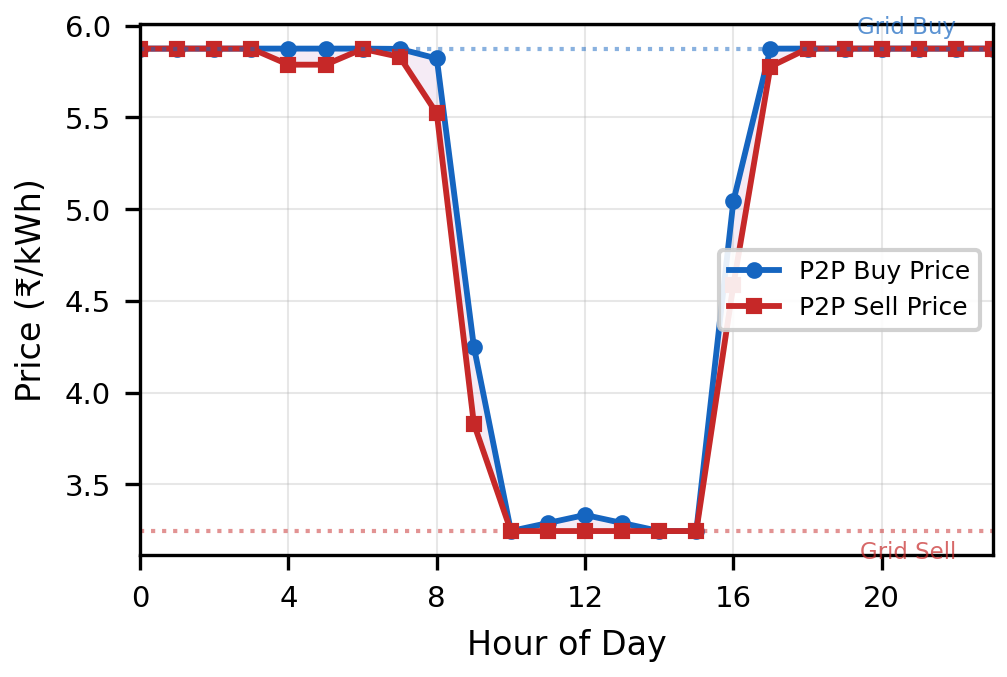
\includegraphics[width=\columnwidth]{fig10.png}
    \caption{Hourly internal P2P market clearing prices compared with grid tariffs.}
    \label{fig:prices}
\end{figure}

\subsection{Comparative Price Analysis}

Fig.~\ref{fig:comparison} compares all the four pricing mechanisms. The SDR-DSM based mechanism exhibits the strongest  responsiveness, with prices collapsing toward $\bar{\pi}^{\text{sell}}$ during surplus and converging toward $\bar{\pi}^{\text{buy}}$ during deficit. Table~\ref{tab:price_comparison} quantifies the differences.

\begin{figure}[t]
    \centering
    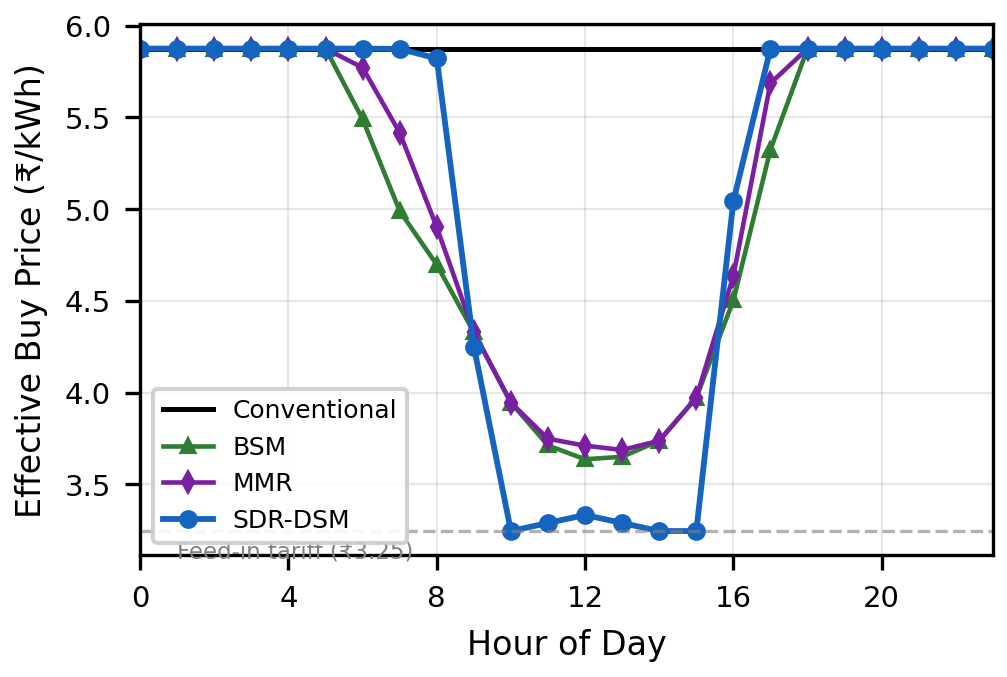
\includegraphics[width=\columnwidth]{fig12.png}
    \caption{Comparative validation of SDR-based P2P trading prices with conventional, BSM, and MMR mechanisms.}
    \label{fig:comparison}
\end{figure}

\begin{table}[t]
\caption{Comparative Intraday Price Extremes and Regime Characteristics}
\label{tab:price_comparison}
\centering
\footnotesize
\begin{tabular}{lcccc}
\toprule
\textbf{Metric} & \textbf{Conv.} & \textbf{BSM} & \textbf{MMR} & \textbf{SDR} \\
\midrule
Max buy (\rupee/kWh) & 5.88 & 5.88 & 5.88 & 5.88 \\
Min sell (\rupee/kWh) & 3.25 & 3.64 & 3.69 & 3.25 \\
Avg midday buy (\rupee/kWh) & 5.88 & 3.86 & 3.88 & 3.41 \\
Price spread (\rupee/kWh) & 2.63 & 2.24 & 2.56 & 2.63 \\
\bottomrule
\end{tabular}
\end{table}

\subsection{Economic Evaluation}

Table~\ref{tab:economics} presents comparative economic outcomes. MMR achieves high consumer savings (19.15\% group-level) but depreciates prosumer revenues by 5.13\%, yielding $\mathcal{F} = 0.00$ (maximally inequitable). Static SDR similarly penalizes prosumers ($-$12.63\%) despite strong consumer benefits. BSM achieves moderate fairness ($\mathcal{F} = 0.67$) but with limited savings. The SDR-DSM framework achieves $\mathcal{F} = 0.80$ alongside 15.35\% community cost reduction, 18.15\% consumer savings, and 11.98\% prosumer revenue enhancement.

To validate configurability, Table~\ref{tab:sweep} presents SDR-DSM results across three additional community sizes ($N=7$ to $N=30$). The framework scales without structural modification, consistently achieving the highest fairness and positive savings for both participant groups across all configurations.

\begin{table}[t]
\caption{30-Day Economic Performance Comparison}
\label{tab:economics}
\centering
\footnotesize
\begin{tabular}{lcccc}
\toprule
\textbf{Metric} & \textbf{BSM} & \textbf{MMR} & \textbf{SDR} & \textbf{SDR-DSM} \\
\midrule
Community savings (\%) & 6.55 & 8.13 & 5.32 & \textbf{15.35} \\
Consumer $\Delta_{\mathcal{C}}$ (\%) & 8.47 & 19.15 & 20.25 & \textbf{18.15} \\
Prosumer $\Delta_{\mathcal{P}}$ (\%) & $+$4.23 & $-$5.13 & $-$12.63 & \textbf{$+$11.98} \\
Fairness $\mathcal{F}$ & 0.67 & 0.00 & 0.00 & \textbf{0.80} \\
\bottomrule
\end{tabular}
\vspace{8pt}
\caption{Community Size Sweep: SDR-DSM Performance}
\label{tab:sweep}
\vspace{4pt}
\begin{tabular}{lcccc}
\toprule
\textbf{Configuration} & \textbf{Savings (\%)} & $\Delta_{\mathcal{C}}$ \textbf{(\%)} & $\Delta_{\mathcal{P}}$ \textbf{(\%)} & $\mathcal{F}$ \\
\midrule
2C + 5P ($N=7$) & 18.55 & 20.35 & 14.72 & 0.84 \\
5C + 15P ($N=20$) & 14.93 & 16.93 & 13.34 & 0.88 \\
10C + 20P ($N=30$) & 13.64 & 15.38 & 11.18 & 0.84 \\
\bottomrule
\end{tabular}
\end{table}

%====================================================================
\section{Conclusion}

This paper presented a modular comparative analysis framework for benchmarking P2P energy trading mechanisms under standardized conditions. Systematic evaluation across community sizes from $N=7$ to $N=30$ revealed that aggregate cost savings and prosumer equity are inversely coupled in MMR and static SDR pricing. For the primary $N=10$ community, SDR-DSM achieves 15.35\% community savings with $\mathcal{F} = 0.80$, compared to MMR which achieves 8.13\% savings but at $\mathcal{F} = 0.00$ due to prosumer penalization. The community size sweep confirms scalability, with SDR-DSM consistently achieving positive savings for both participant groups across all configurations tested.

Future work will extend the framework with ACOPF network constraints, stochastic optimization for forecast uncertainty, and BESS/V2G modules for temporal energy arbitrage.

\vfill\eject
\bibliographystyle{IEEEtran}

{\footnotesize
\begin{thebibliography}{00}

\bibitem{irena2025}
IRENA, ``Renewable capacity statistics 2025,'' International Renewable Energy Agency, Abu Dhabi, 2025.

\bibitem{sousa2019}
T. Sousa \textit{et al.}, ``Peer-to-peer and community-based markets: A comprehensive review,'' \textit{Renew. Sustain. Energy Rev.}, vol.~104, pp.~367--378, 2019.

\bibitem{zhou2023}
Y. Zhou and P. D. Lund, ``Peer-to-peer energy sharing and trading of renewable energy in smart communities,'' \textit{Renew. Energy}, vol.~207, pp.~177--193, 2023.

\bibitem{domenech2022}
M. Dom\`{e}nech Monfort \textit{et al.}, ``A review of peer-to-peer energy trading with standard terminology proposal,'' \textit{Energies}, vol.~15, no.~23, p.~9070, 2022.

\bibitem{long2017}
C. Long, J. Wu, C. Zhang, M. Cheng, and A. Al-Wakeel, ``Peer-to-peer energy trading in a community microgrid,'' in \textit{Proc. IEEE PES Gen. Meeting}, 2017, pp.~1--5.

\bibitem{zhang2018}
C. Zhang, J. Wu, Y. Zhou, M. Cheng, and C. Long, ``Peer-to-peer energy trading in a microgrid,'' \textit{Appl. Energy}, vol.~220, pp.~1--12, 2018.

\bibitem{huang2025}
W. Huang \textit{et al.}, ``Auction-based P2P energy trading mechanisms,'' \textit{Appl. Energy}, 2025.

\bibitem{zhang2024}
C. Zhang \textit{et al.}, ``Auction-based peer-to-peer energy trading considering echelon utilization of retired EV batteries,'' \textit{Appl. Energy}, vol.~358, p.~122592, 2024.

\bibitem{liaquat2023a}
S. Liaquat \textit{et al.}, ``Comparative analysis of peer-to-peer PV trading strategies under network constraints,'' \textit{Appl. Sci.}, vol.~13, no.~18, p.~10044, 2023.

\bibitem{long2019}
C. Long, Y. Zhou, and J. Wu, ``A game theoretic approach for peer to peer energy trading,'' \textit{Energy Procedia}, vol.~159, pp.~454--459, 2019.

\bibitem{tushar2019}
W. Tushar \textit{et al.}, ``A motivational game-theoretic approach for peer-to-peer energy trading in the smart grid,'' \textit{Appl. Energy}, vol.~243, pp.~10--20, 2019.

\bibitem{bogensperger2021}
A. Bogensperger, J. Ferstl, and Y. Yu, ``Comparison of pricing mechanisms in peer-to-peer energy communities,'' in \textit{Proc. Int. Energiewirtschaftstagung}, 2021, p.~12.

\bibitem{teotia2020}
F. Teotia, P. Mathuria, and R. Bhakar, ``Peer-to-peer local electricity market platform pricing strategies,'' \textit{IET Gener. Transm. Distrib.}, vol.~14, no.~20, pp.~4388--4397, 2020.

\bibitem{alfaverh2023}
F. Alfaverh, M. Denai, and Y. Sun, ``A dynamic peer-to-peer electricity market model for a community microgrid with price-based demand response,'' \textit{IEEE Trans. Smart Grid}, vol.~14, no.~5, pp.~3976--3991, 2023.

\bibitem{dwivedi2022}
D. Dwivedi \textit{et al.}, ``Evaluation of energy resilience and cost benefit in microgrid with peer-to-peer energy trading,'' \textit{arXiv:2212.02318}, 2022.

\bibitem{liu2017}
N. Liu \textit{et al.}, ``Energy-sharing model with price-based demand response for microgrids of peer-to-peer prosumers,'' \textit{IEEE Trans. Power Syst.}, vol.~32, no.~5, pp.~3569--3583, 2017.




\end{thebibliography}}

\end{document}
